\chapter{参考：クロスドメイン技術候補抽出研究の図表}
\label{ch:crossdomain}

本章では、参考として、クロスドメイン技術候補抽出に関する研究で生成された図表を示す。この研究は、特許文書から課題文脈と解決手段文脈を分離し、異分野間における技術候補を抽出する手法を提案している。

\section{候補タイプの定義と実験の位置づけ}
図 \ref{fig:reference_solution_type_quadrant} に、課題文脈類似度と解決手段文脈類似度に基づく候補タイプの概念図を示す。この図では、実験1（近接解決策型）と実験2（異質解決策型）の位置づけが明確に示されている。

\begin{figure}[htbp]
\begin{center}
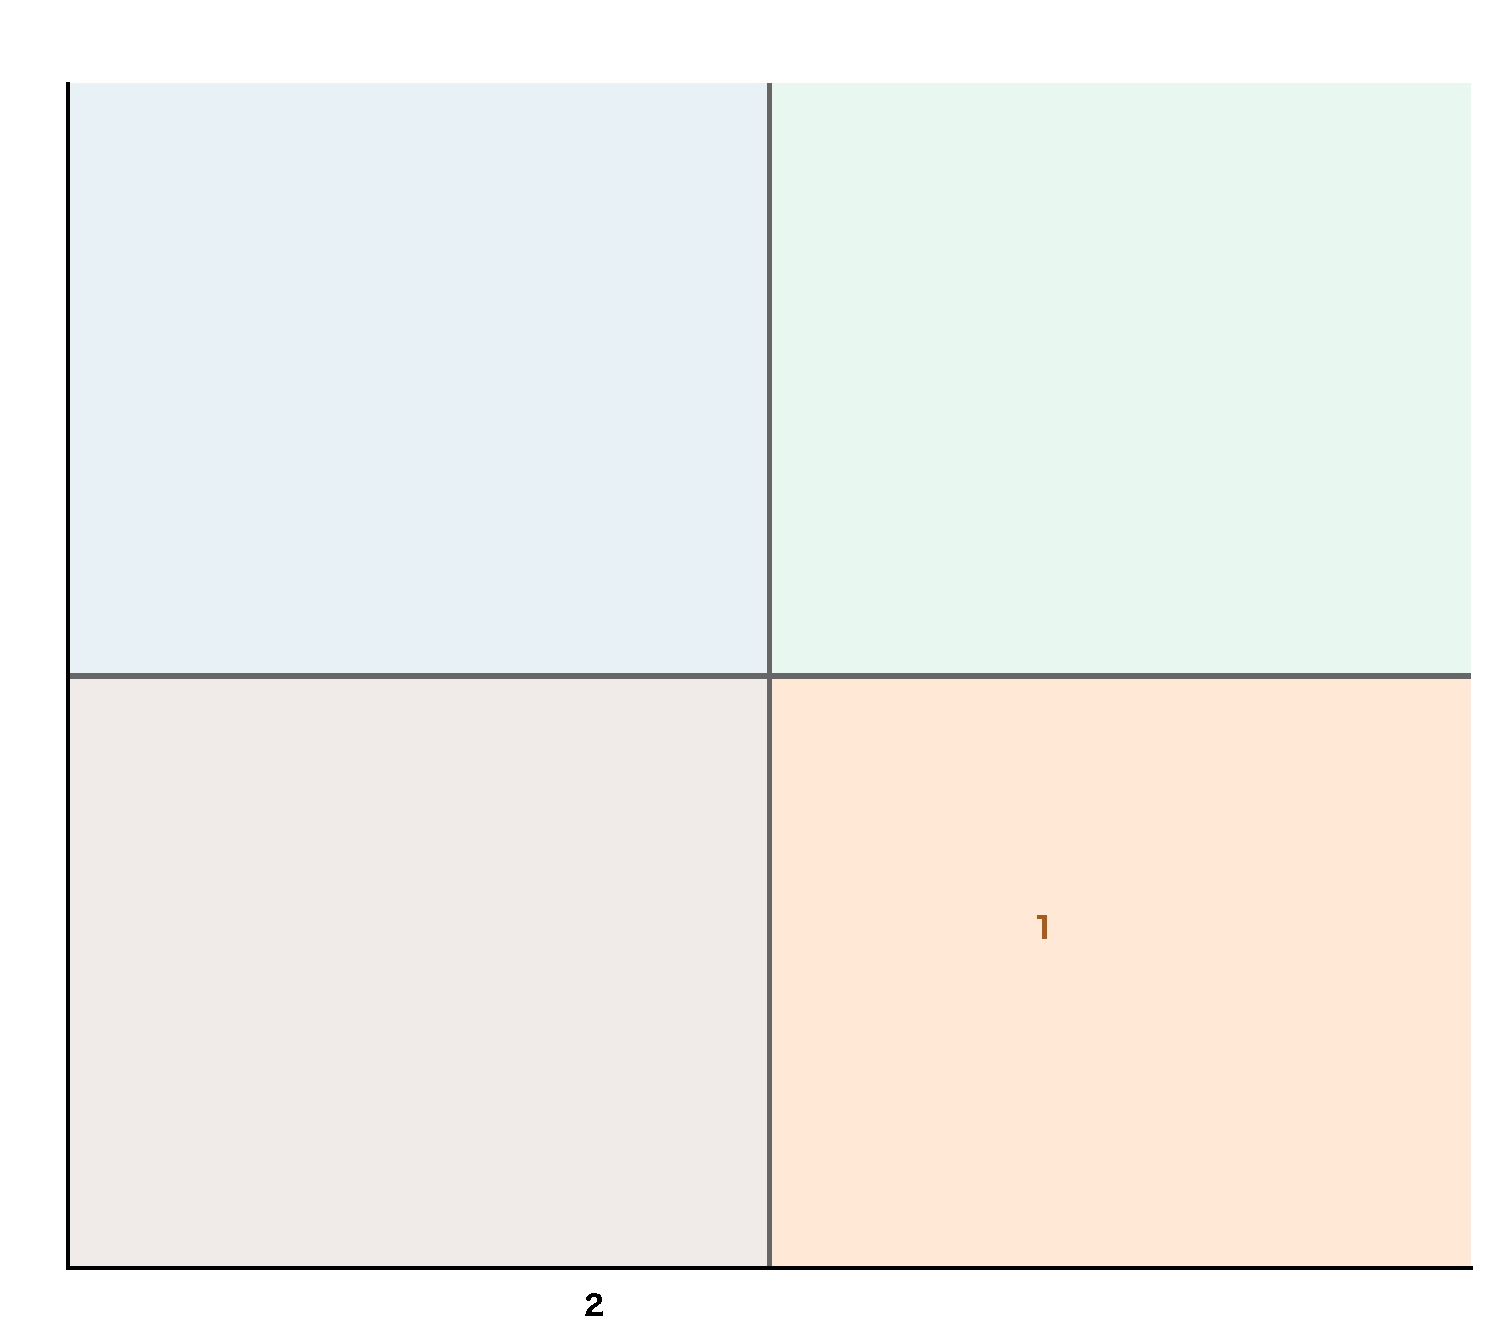
\includegraphics[width=0.85\textwidth]{figures/solution_type_quadrant.pdf}
\caption{候補タイプと実験の位置づけ}
\label{fig:reference_solution_type_quadrant}
\end{center}
\end{figure}

\section{提案手法の処理フロー}
図 \ref{fig:reference_method_pipeline} に、提案手法全体の処理フローを示す。特許データから候補集合の抽出、著者確認評価に至るまでの一連のプロセスが可視化されている。

\begin{figure}[htbp]
\begin{center}
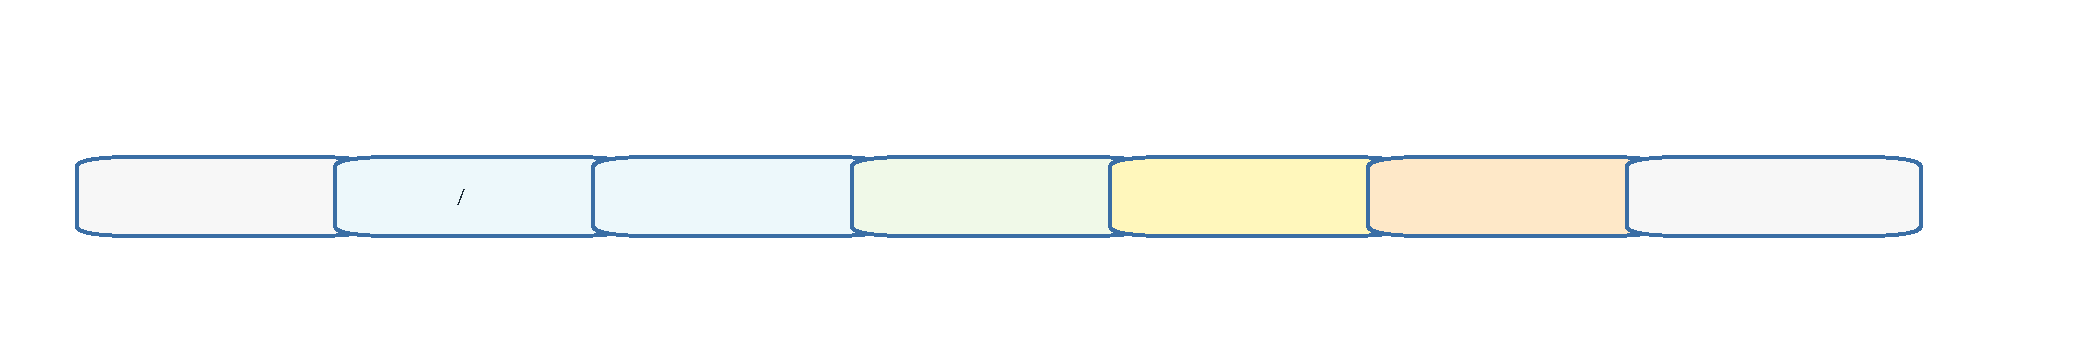
\includegraphics[width=0.95\textwidth]{figures/method_pipeline.pdf}
\caption{提案手法の全体処理フロー}
\label{fig:reference_method_pipeline}
\end{center}
\end{figure}

\section{実験1：U-Net候補抽出フロー}
図 \ref{fig:reference_experiment1_pipeline} に、実験1の処理フローを示す。医療画像解析分野から製造欠陥検出分野への U-Net 関連候補抽出のプロセスが示されている。

\begin{figure}[htbp]
\begin{center}
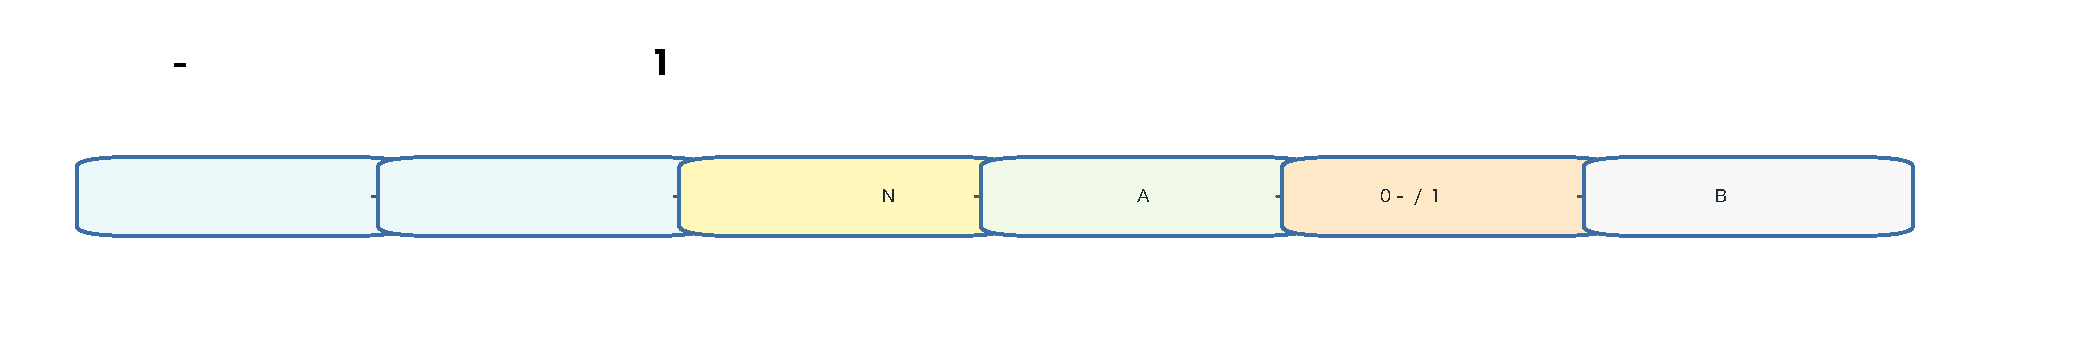
\includegraphics[width=0.95\textwidth]{figures/experiment1_pipeline.pdf}
\caption{実験1フロー：U-Netを対象とした近接解決策型}
\label{fig:reference_experiment1_pipeline}
\end{center}
\end{figure}

\section{実験2：異質解決策型分析フロー}
図 \ref{fig:reference_experiment2_pipeline} に、実験2の処理フローを示す。洗浄・除去系技術を対象とした異質解決策型候補抽出のプロセスが可視化されている。

\begin{figure}[htbp]
\begin{center}
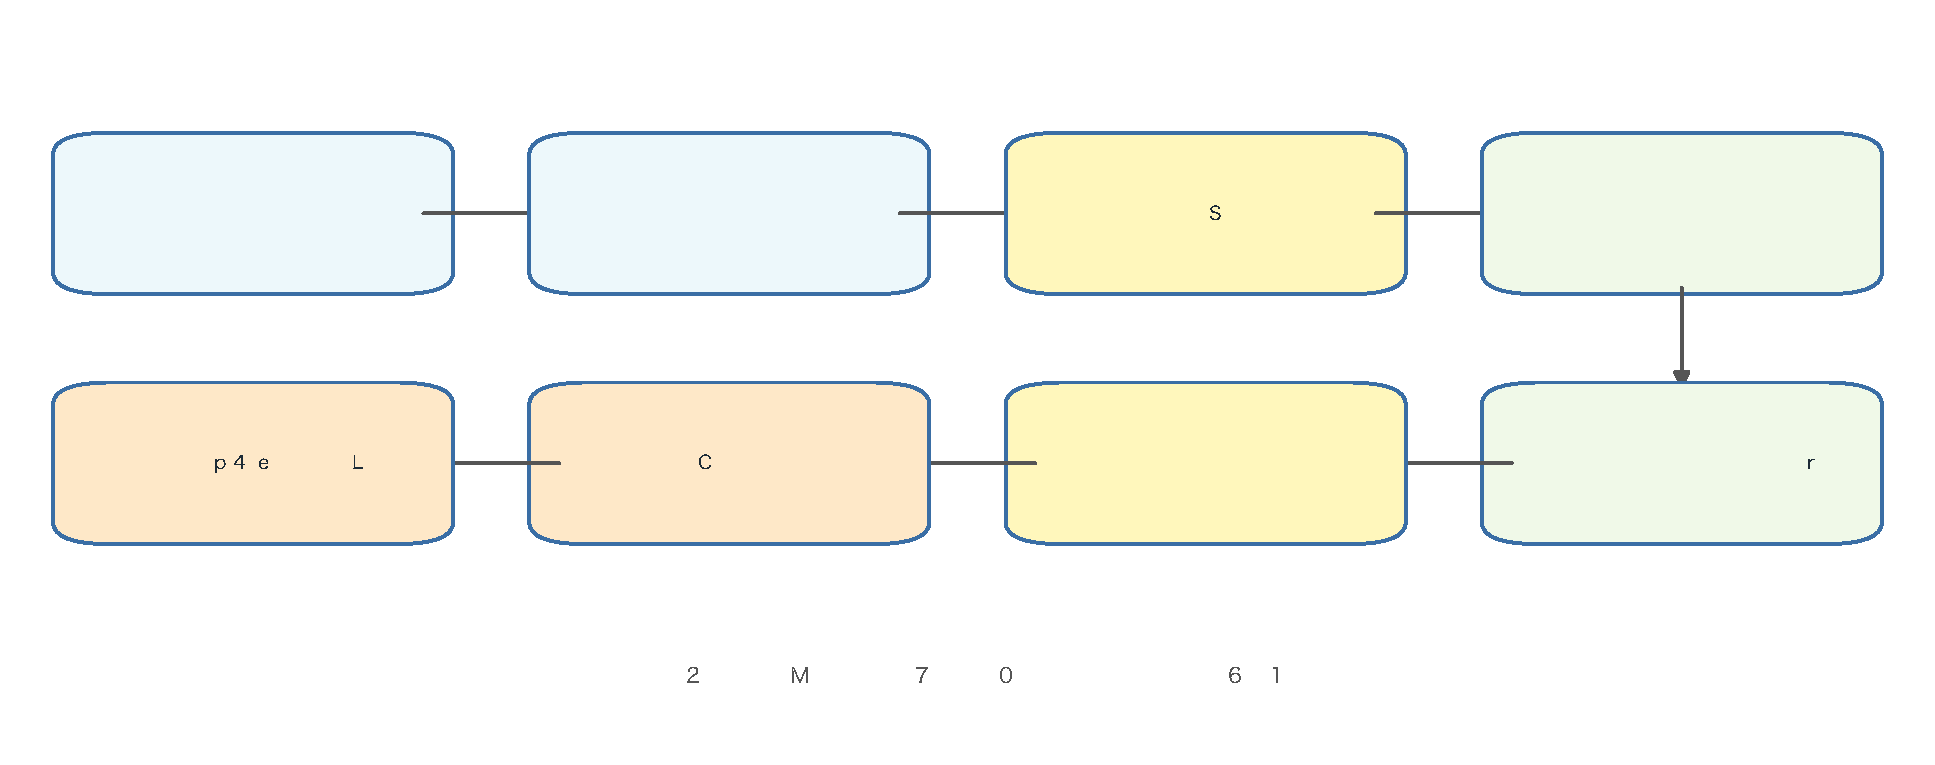
\includegraphics[width=0.95\textwidth]{figures/experiment2_pipeline.pdf}
\caption{実験2フロー：異質解決策型の補助分析}
\label{fig:reference_experiment2_pipeline}
\end{center}
\end{figure}

\section{実験1のU-Net候補抽出結果}
実験1では、医療画像解析分野（A0）から製造欠陥検出分野（B0）への U-Net 関連候補抽出を実施した。データセットは過去・将来期間で分割され、過去のU-Net関連特許からベースラインを構築し、将来期間における候補抽出の有効性を検証した。提案手法による候補ランキングと従来の全文類似度ベースラインを比較し、候補集合の性質の違いを分析した。

\section{実験2の異質解決策型分析}
実験2では、洗浄・除去系技術を対象とした異質解決策型分析を実施した。半導体洗浄課題に関連する複数の用途クラスタを設計し、各クラスタにおける候補抽出を行った。この分析は補助分析として位置づけられ、異質解決策型における候補の解釈可能性を探索的に検証した。

